\chapter{Conception du syst\`eme}
\label{chap:conception-systeme}

\section{Introduction}

La conception relie chaque observation à sa prédiction et, le cas échéant, à
une alerte. Elle prévoit aussi la reprise des traitements interrompus et la
publication des résultats enregistrés. Les diagrammes utilisent les noms
techniques du code pour faciliter le passage du modèle à l'implémentation.

\section{Mod\'elisation statique}

\subsection{Mod\`ele du domaine}

La figure~\ref{fig:domain-classes} relie les observations de flux, les prédictions,
les alertes, les jeux de données et les modèles. Les vues suivantes détaillent
les travaux d'ingestion et le suivi des modèles. Les attributs sont présentés
sans indication de visibilité; le signe \texttt{+} désigne les opérations
publiques des services.

\begin{figure}[htbp]
  \centering
  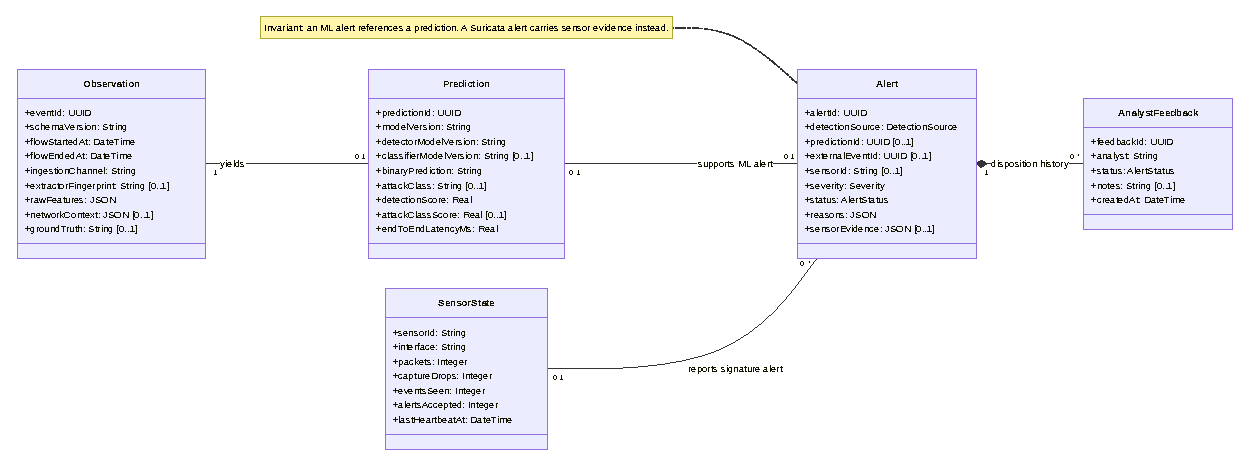
\includegraphics[width=\textwidth,height=0.68\textheight,keepaspectratio]{../diagrams/rendered/03-domain-classes.pdf}
  \caption{Diagramme de classes du domaine principal}
  \label{fig:domain-classes}
\end{figure}

\begin{figure}[htbp]
  \centering
  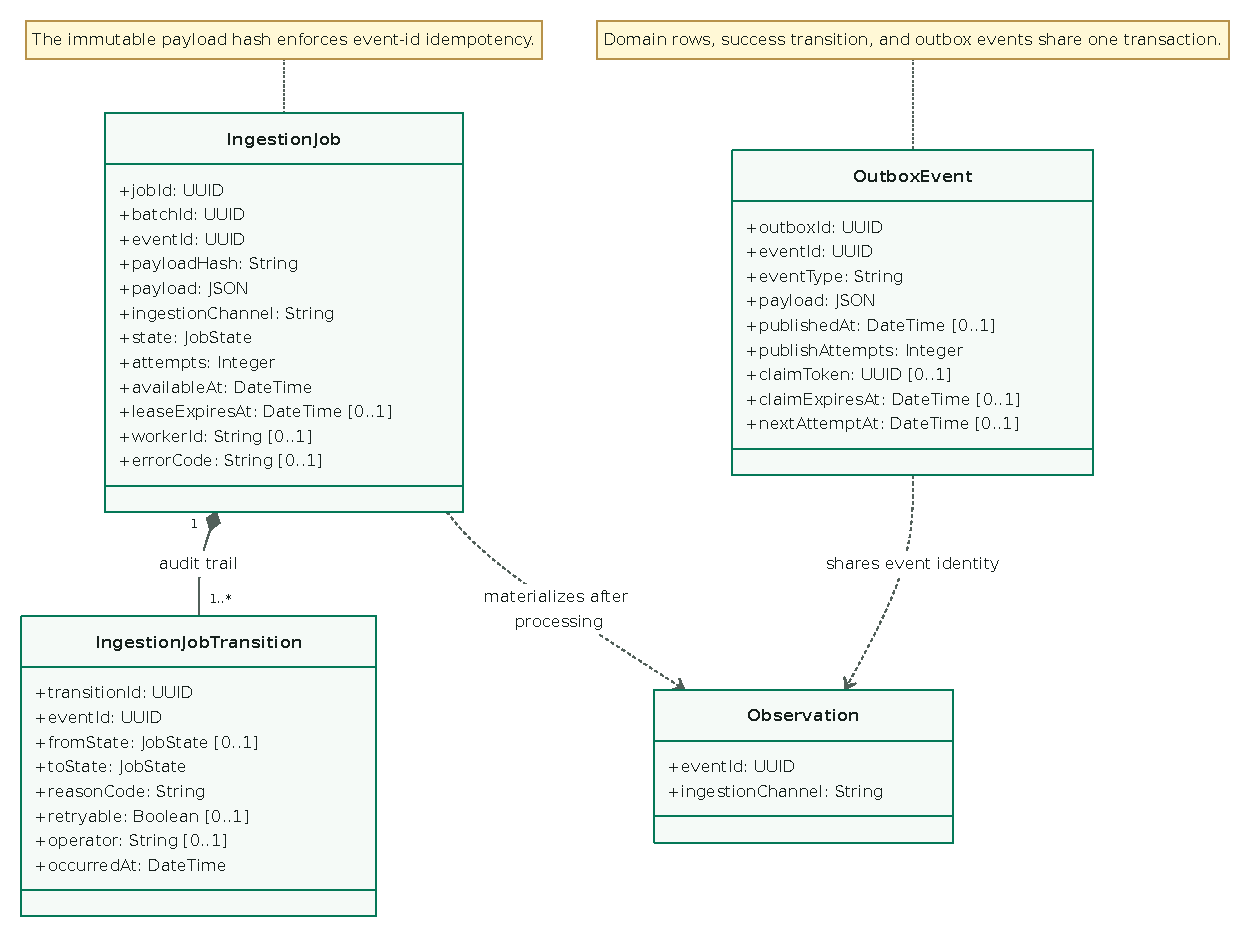
\includegraphics[width=\textwidth,height=0.68\textheight,keepaspectratio]{../diagrams/rendered/03b-ingestion-classes.pdf}
  \caption{Classes associ\'ees à l'ingestion durable}
  \label{fig:ingestion-classes}
\end{figure}

\begin{figure}[htbp]
  \centering
  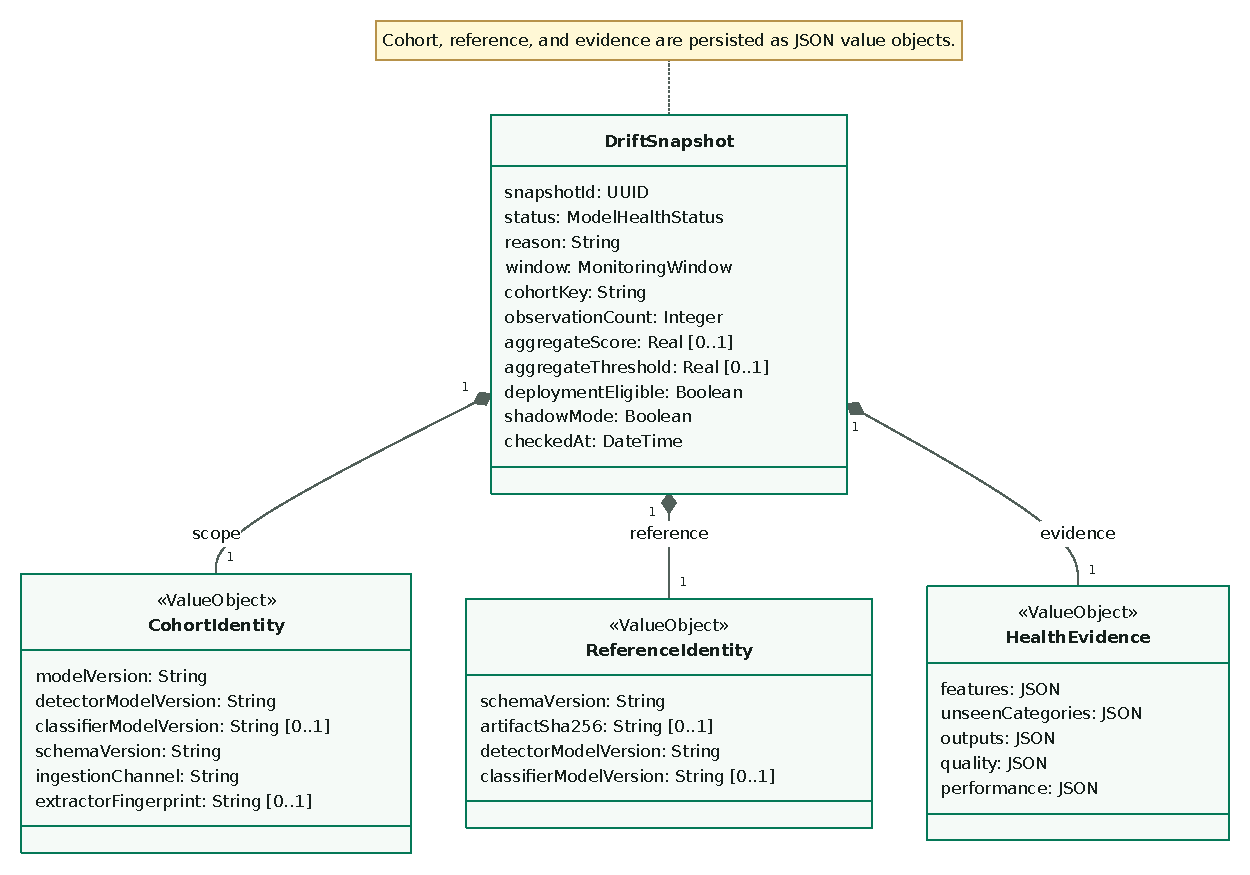
\includegraphics[width=\textwidth,height=0.68\textheight,keepaspectratio]{../diagrams/rendered/03c-model-health-classes.pdf}
  \caption{Classes associ\'ees au suivi de l'\'etat des mod\`eles}
  \label{fig:model-health-classes}
\end{figure}

Les entit\'es persistantes portent les donn\'ees et leurs associations. Les
op\'erations sont volontairement regroup\'ees dans les services qui ex\'ecutent
les transactions et les r\`egles m\'etier. La figure~\ref{fig:service-operations}
présente leurs principales opérations publiques.

\clearpage
\begin{figure}[htbp]
  \centering
  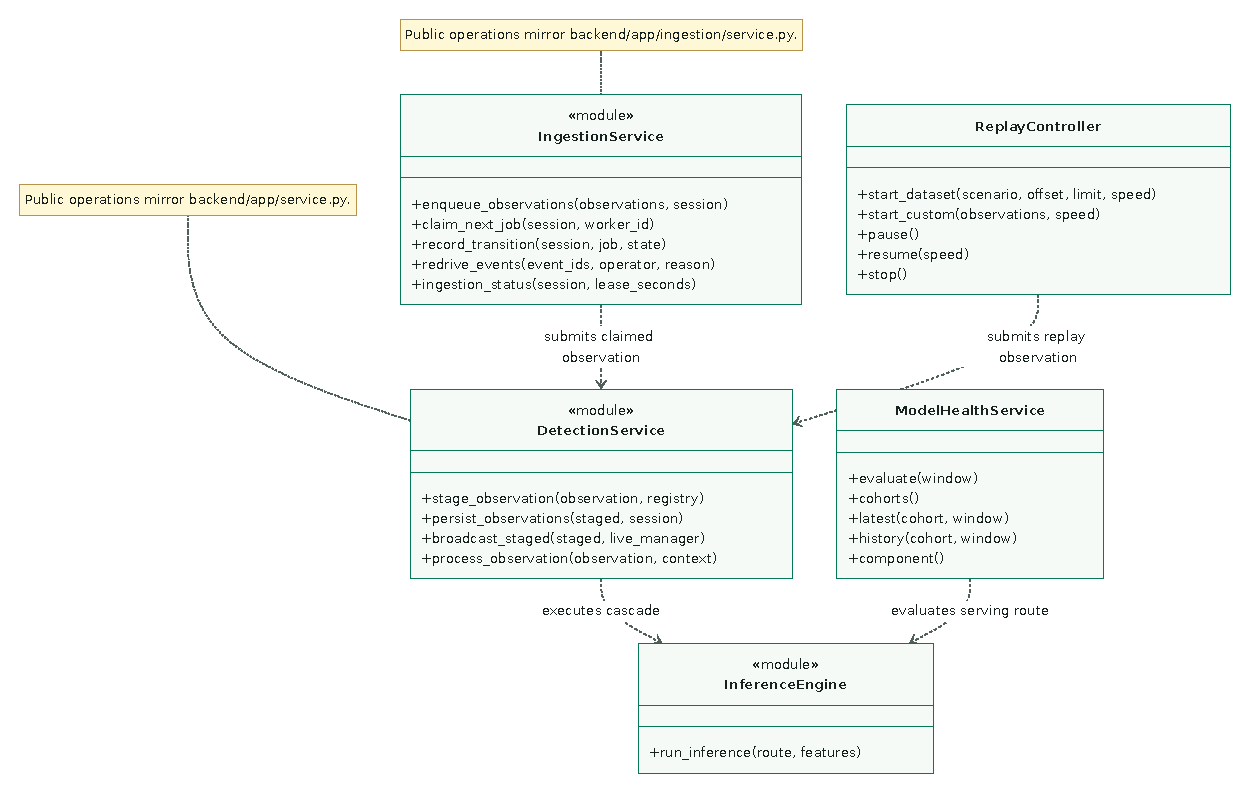
\includegraphics[width=\textwidth,height=0.68\textheight,keepaspectratio]{../diagrams/rendered/03d-service-operations.pdf}
  \caption{Services et op\'erations principales}
  \label{fig:service-operations}
\end{figure}


\subsection{Mod\`ele relationnel}

Le mod\`ele relationnel traduit les classes persistantes en tables. Une
observation poss\`ede une cl\'e primaire \texttt{event\_id}; une pr\'ediction lui
est associ\'ee par une cl\'e \`etrang\`ere unique. Une alerte peut provenir d'une
pr\'ediction ML ou d'un capteur Suricata. Les travaux d'ingestion, leurs
transitions et les messages d'outbox sont s\'epar\'es afin de conserver
l'idempotence, l'historique et la publication apr\`es transaction.

La r\`egle de passage est la suivante : chaque entit\'e devient une table,
chaque identifiant devient une cl\'e primaire, les relations un-\`a-un utilisent
une cl\'e \`etrang\`ere unique et les relations un-\`a-plusieurs placent la cl\'e
\`etrang\`ere du c\^ot\'e plusieurs. Les objets JSON regroupent les attributs
variables dont la structure dépend du type d'observation ou de preuve.

\subsection{Dictionnaire de donn\'ees}

Le dictionnaire suivant reprend les champs principaux du mod\`ele. Les champs
JSON contiennent les caract\'eristiques ou les preuves variables; les colonnes
de statut et d'identit\'e sont contr\^ol\'ees par les contrats et contraintes du
backend.

\begin{table}[!t]
  \centering
  \small
  \renewcommand{\arraystretch}{1.14}
  \caption{Dictionnaire synthétique des données persistées}
  \label{tab:data-dictionary}
  \begin{tabularx}{\textwidth}{@{}>{\raggedright\arraybackslash}p{0.18\textwidth}>{\raggedright\arraybackslash}p{0.25\textwidth}>{\raggedright\arraybackslash}p{0.18\textwidth}Y@{}}
  \rowcolor{PremiumEmerald}\color{white}\bfseries Table & \color{white}\bfseries Colonne & \color{white}\bfseries Type / taille & \color{white}\bfseries Contraintes et rôle \\
  observations & event\_id & UUID / 36 & clé primaire, obligatoire \\
  observations & schema\_version & texte / 64 & obligatoire, contrat versionné \\
  observations & raw\_features & JSON & obligatoire, 83 variables validées \\
  observations & network\_context & JSON & facultatif, contexte réseau \\
  predictions & prediction\_id & UUID / 36 & clé primaire \\
  predictions & event\_id & UUID / 36 & clé étrangère unique vers observations \\
  predictions & detector\_model\_version & texte / 128 & obligatoire, artefact servi \\
  predictions & binary\_prediction & texte / 16 & obligatoire, normal ou attack \\
  alerts & alert\_id & UUID / 36 & clé primaire \\
  alerts & detection\_source & texte / 32 & obligatoire, ML ou Suricata \\
  alerts & prediction\_id & UUID / 36 & clé étrangère facultative et unique \\
  ingestion\_jobs & event\_id & UUID / 36 & unique, clé d'idempotence \\
  ingestion\_jobs & state & texte / 24 & état du cycle de traitement \\
  outbox\_events & event\_id & UUID / 36 & identité de publication \\
  \bottomrule
  \end{tabularx}
\end{table}

\clearpage
\section{Architecture de l'application}

La figure~\ref{fig:component-architecture} situe l'interface, les services de
l'API, la cascade et la base de données. La file de traitement et l'outbox
utilisent cette base. L'outbox est une table de messages à publier, écrits dans
la même transaction que les résultats auxquels ils se rapportent.

\begin{figure}[!htbp]
  \centering
  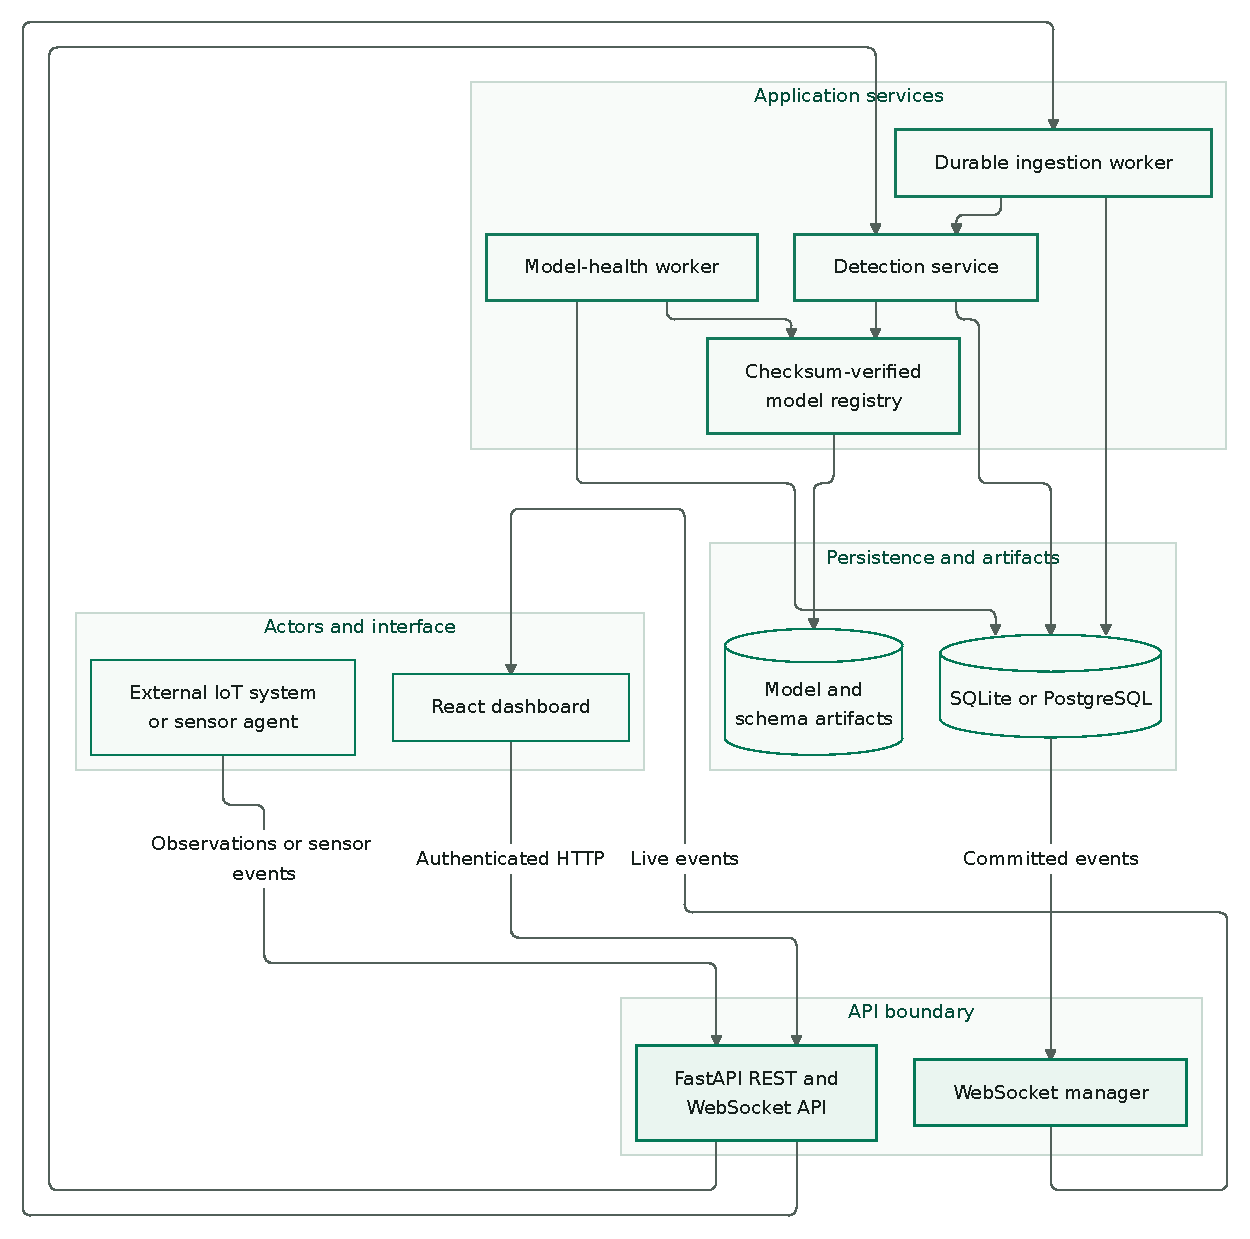
\includegraphics[width=0.98\textwidth,height=0.58\textheight,keepaspectratio]{../diagrams/rendered/14-component-architecture.pdf}
  \caption{Architecture logicielle par composants}
  \label{fig:component-architecture}
\end{figure}

La figure~\ref{fig:docker-deployment} repr\'esente uniquement le mode de
d\'emonstration Docker Compose: une passerelle web, l'API, le travailleur, la
migration et PostgreSQL. Le laboratoire Suricata isol\'e reste un environnement
de pr\'esentation distinct.

\clearpage
\noindent\begin{minipage}{\textwidth}
  \centering
  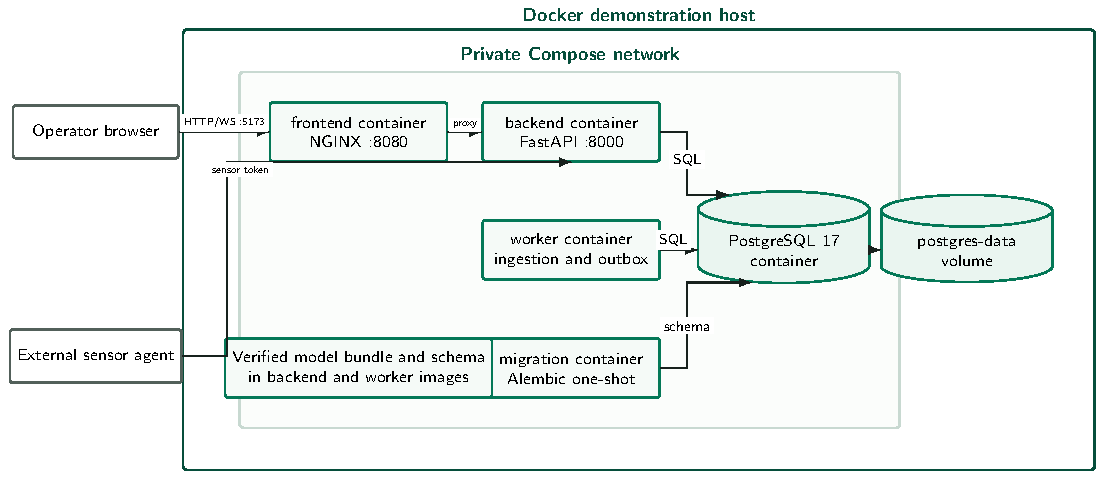
\includegraphics[width=0.98\textwidth,height=0.72\textheight,keepaspectratio]{../diagrams/rendered/15-docker-deployment.pdf}
  \captionof{figure}{D\'eploiement du mode de d\'emonstration Docker}
  \label{fig:docker-deployment}
\end{minipage}

\clearpage
\section{Mod\'elisation dynamique}

Les diagrammes dynamiques suivent les actions de l'opérateur puis les échanges
entre services. La machine à états détaille le cycle de traitement d'une
observation acceptée dans la file.

\subsection{Activit\'e de l'op\'erateur}

Depuis la supervision, l'opérateur peut lancer un rejeu, consulter une alerte
ou examiner les modèles. La figure~\ref{fig:operator-activity} présente ces
choix et les étapes de l'investigation.

\begin{figure}[!htbp]
  \centering
  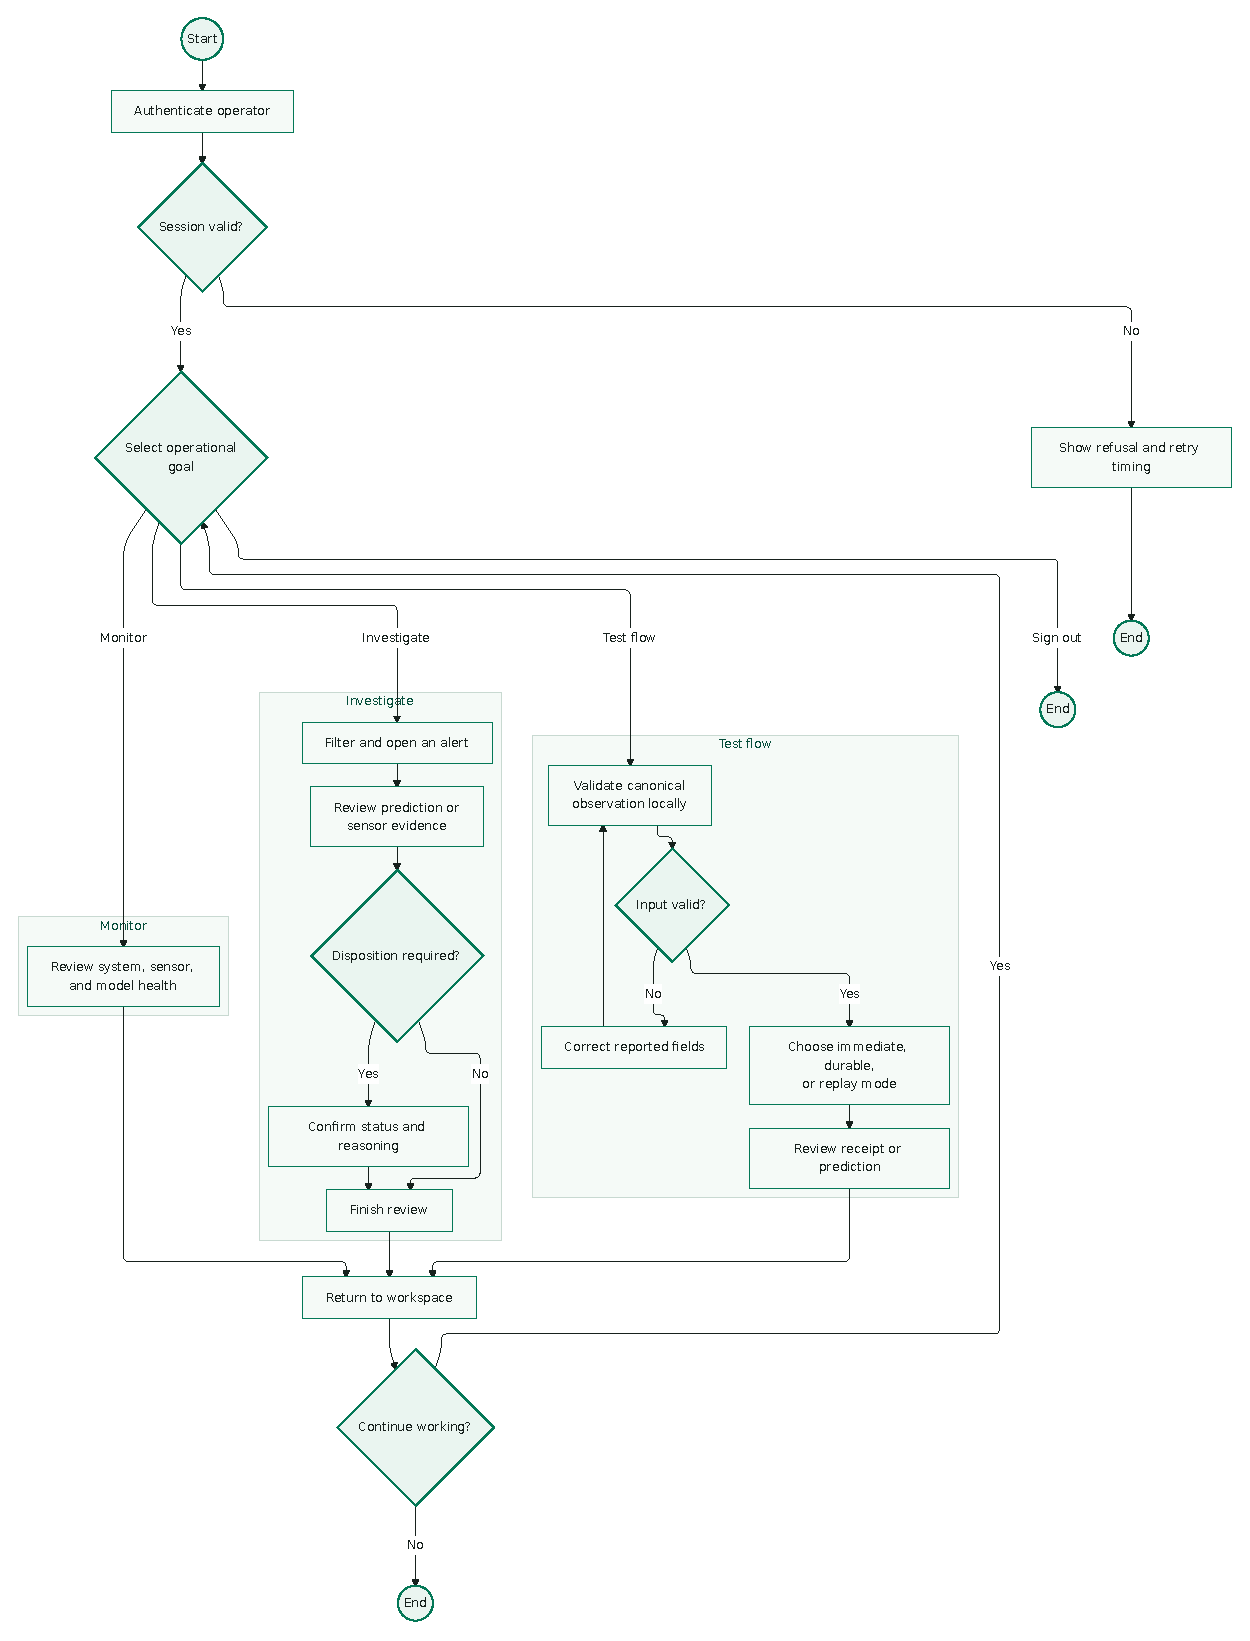
\includegraphics[width=0.98\textwidth,height=0.72\textheight,keepaspectratio]{../diagrams/rendered/12-operator-activity.pdf}
  \caption{Activit\'e principale de l'op\'erateur}
  \label{fig:operator-activity}
\end{figure}

\subsection{Communication pendant l'investigation}

La figure~\ref{fig:alert-communication} montre les objets sollicités pendant
l'examen d'une alerte. Les numéros donnent l'ordre des messages, de la demande
de détail à l'enregistrement de la qualification.

\begin{figure}[!htbp]
  \centering
  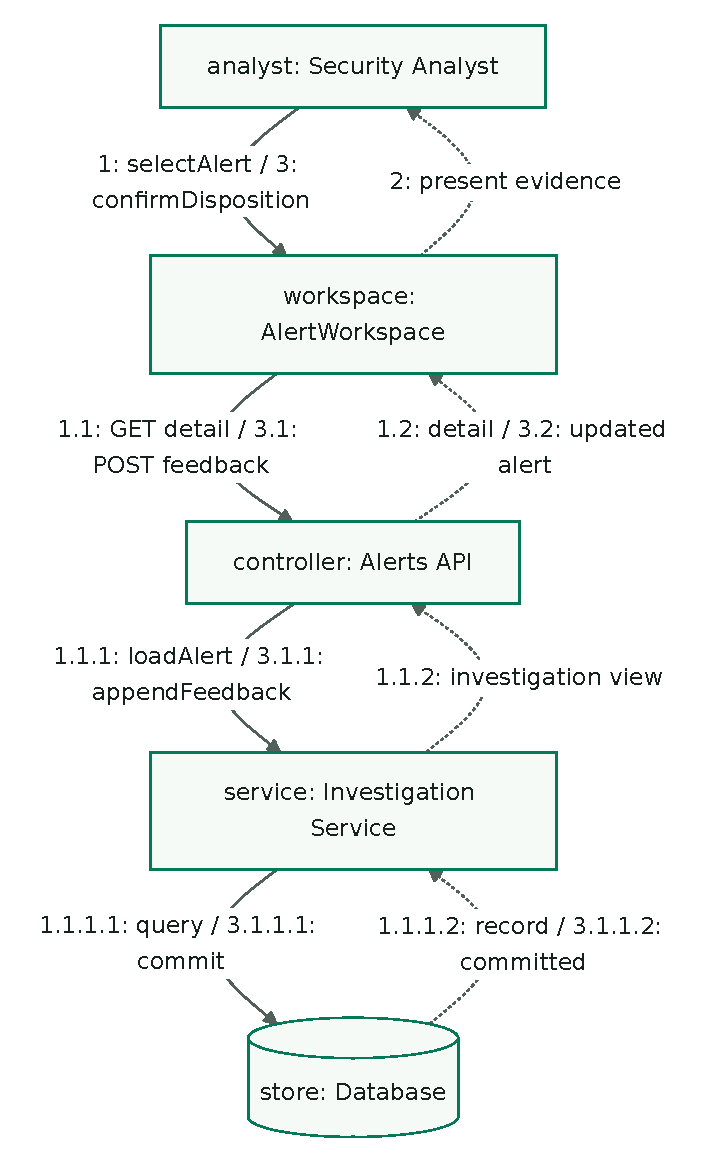
\includegraphics[width=\textwidth,height=0.62\textheight,keepaspectratio]{../diagrams/rendered/13-alert-communication.pdf}
  \caption{Communication entre objets lors de l'investigation d'une alerte}
  \label{fig:alert-communication}
\end{figure}

\subsection{Ingestion durable des observations}

La figure~\ref{fig:ingestion-sequence} s\'epare l'acceptation HTTP, le traitement
asynchrone et la diffusion temps r\'eel. Les transactions rendent visibles les
fronti\`eres d'atomicit\'e, tandis que les fragments alternatifs explicitent le
rejet, la r\'eussite et la reprise apr\`es erreur. Le cycle de vie persistant
correspondant est synth\'etis\'e par la figure~\ref{fig:ingestion-states}.

\begin{figure}[!htbp]
  \centering
  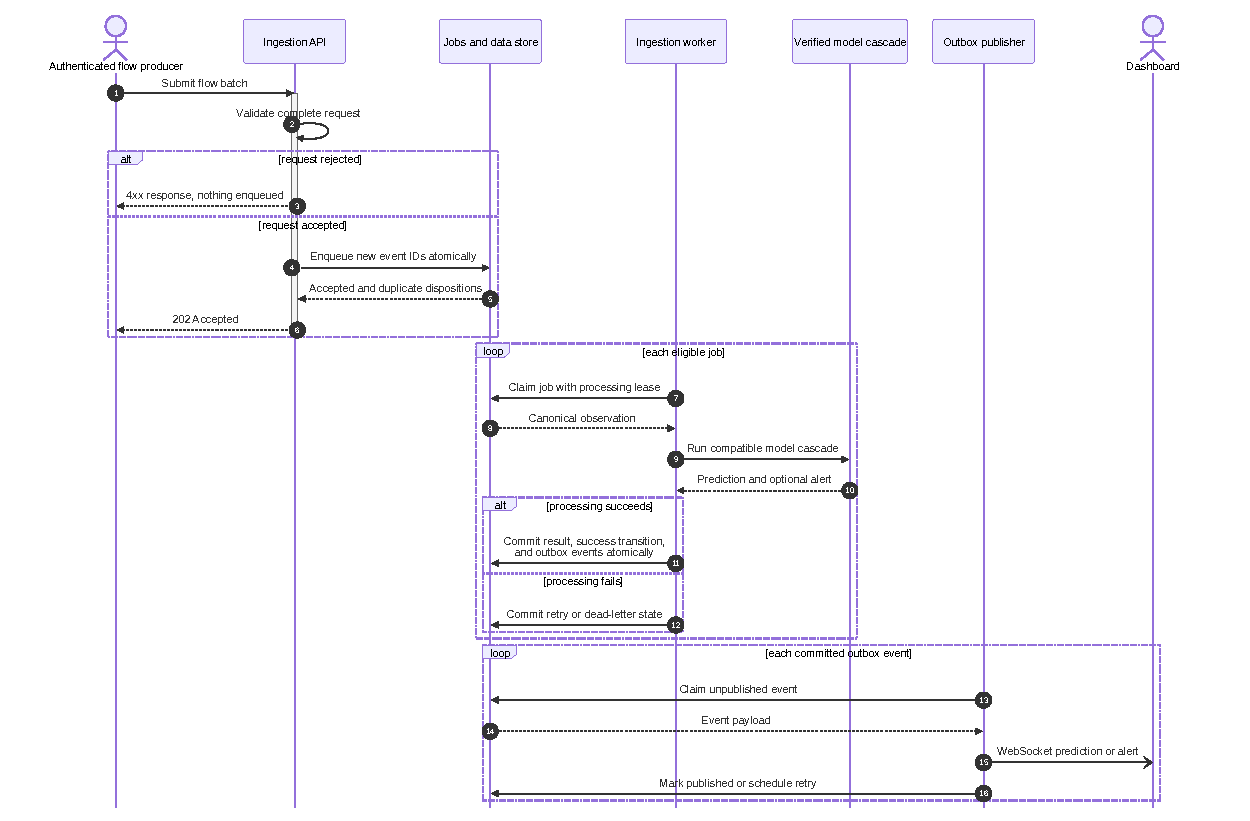
\includegraphics[width=\textwidth,height=0.68\textheight,keepaspectratio]{../diagrams/rendered/02-ingestion-sequence.pdf}
  \caption{S\'equence d'ingestion durable et de diffusion des r\'esultats}
  \label{fig:ingestion-sequence}
\end{figure}

\begin{figure}[!htbp]
  \centering
  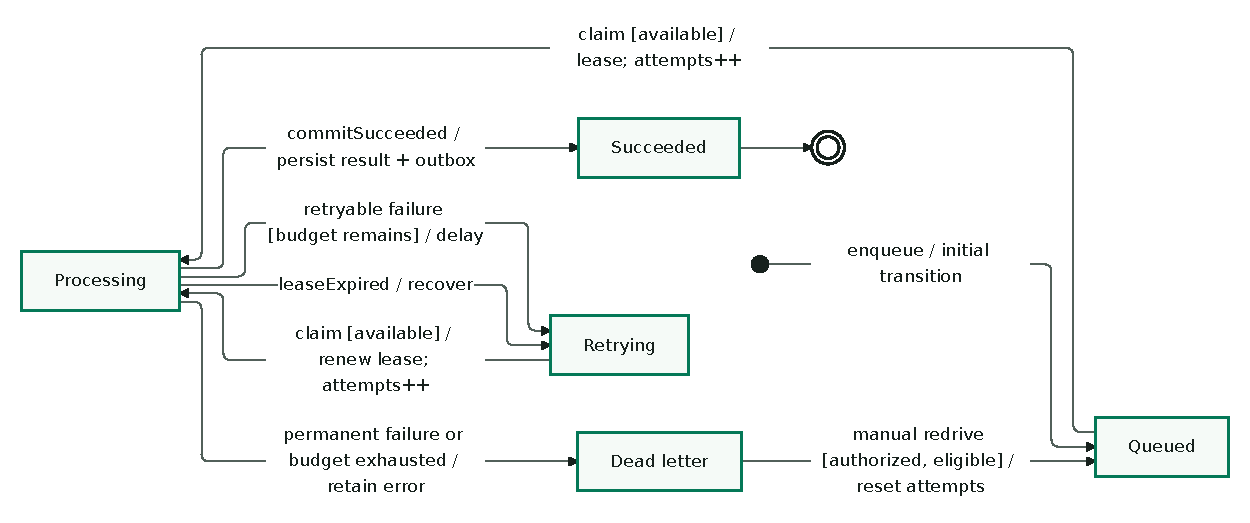
\includegraphics[width=0.98\textwidth,height=0.52\textheight,keepaspectratio]{../diagrams/rendered/04-ingestion-states.pdf}
  \caption{Machine à \'etats d'un travail d'ingestion}
  \label{fig:ingestion-states}
\end{figure}

\clearpage
\subsection{Pr\'ediction synchrone}

Dans le parcours synchrone, l'API valide le schéma, charge une cascade compatible
et exécute l'inférence. Elle enregistre ensuite les résultats dans une
transaction avant de répondre au client
(figure~\ref{fig:synchronous-prediction}).

\begin{figure}[htbp]
  \centering
  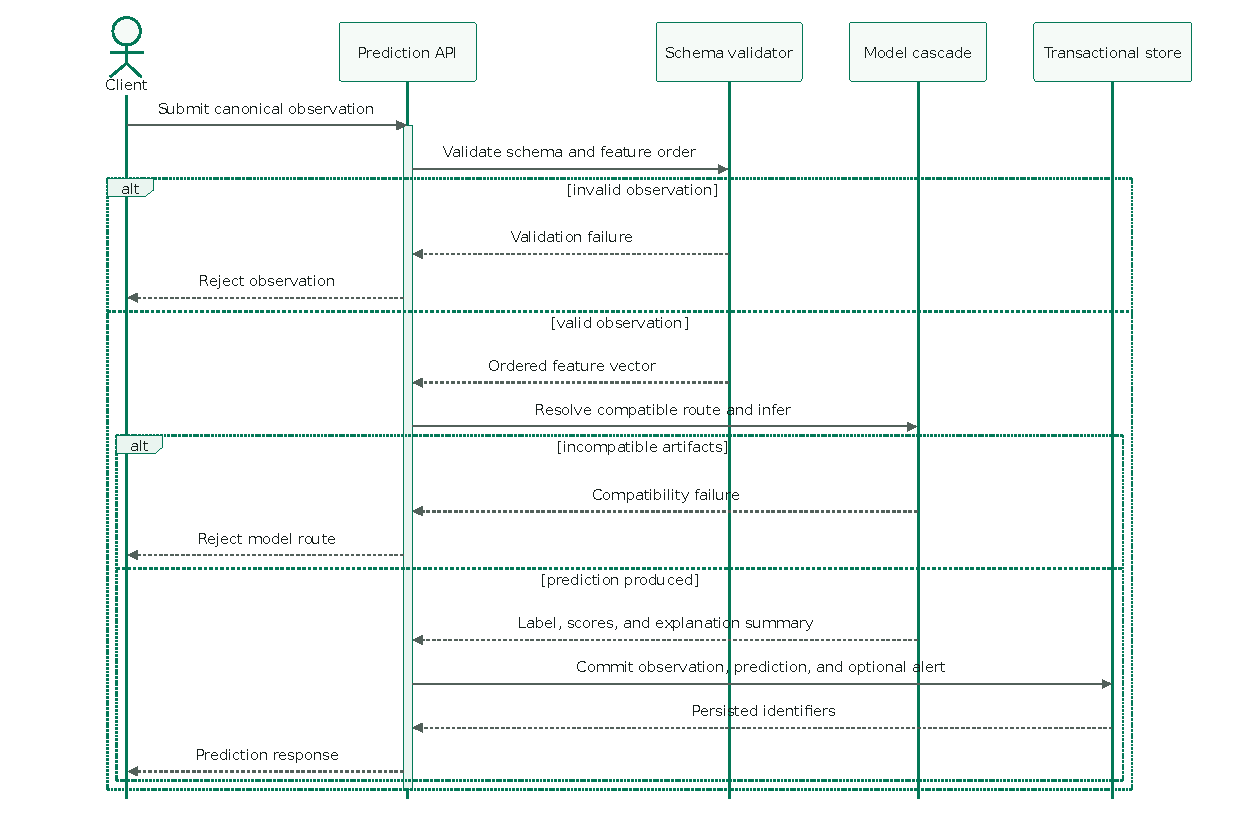
\includegraphics[width=\textwidth,height=0.68\textheight,keepaspectratio]{../diagrams/rendered/07-synchronous-prediction-sequence.pdf}
  \caption{S\'equence de pr\'ediction synchrone}
  \label{fig:synchronous-prediction}
\end{figure}

\clearpage
\subsection{Investigation des alertes}

L'investigation d'une alerte est d\'etaill\'ee dans la
figure~\ref{fig:alert-investigation}. Elle relie la consultation des preuves à
la d\'ecision de l'analyste et conserve une trace de l'interpr\'etation humaine
du r\'esultat automatique.

\begin{figure}[htbp]
  \centering
  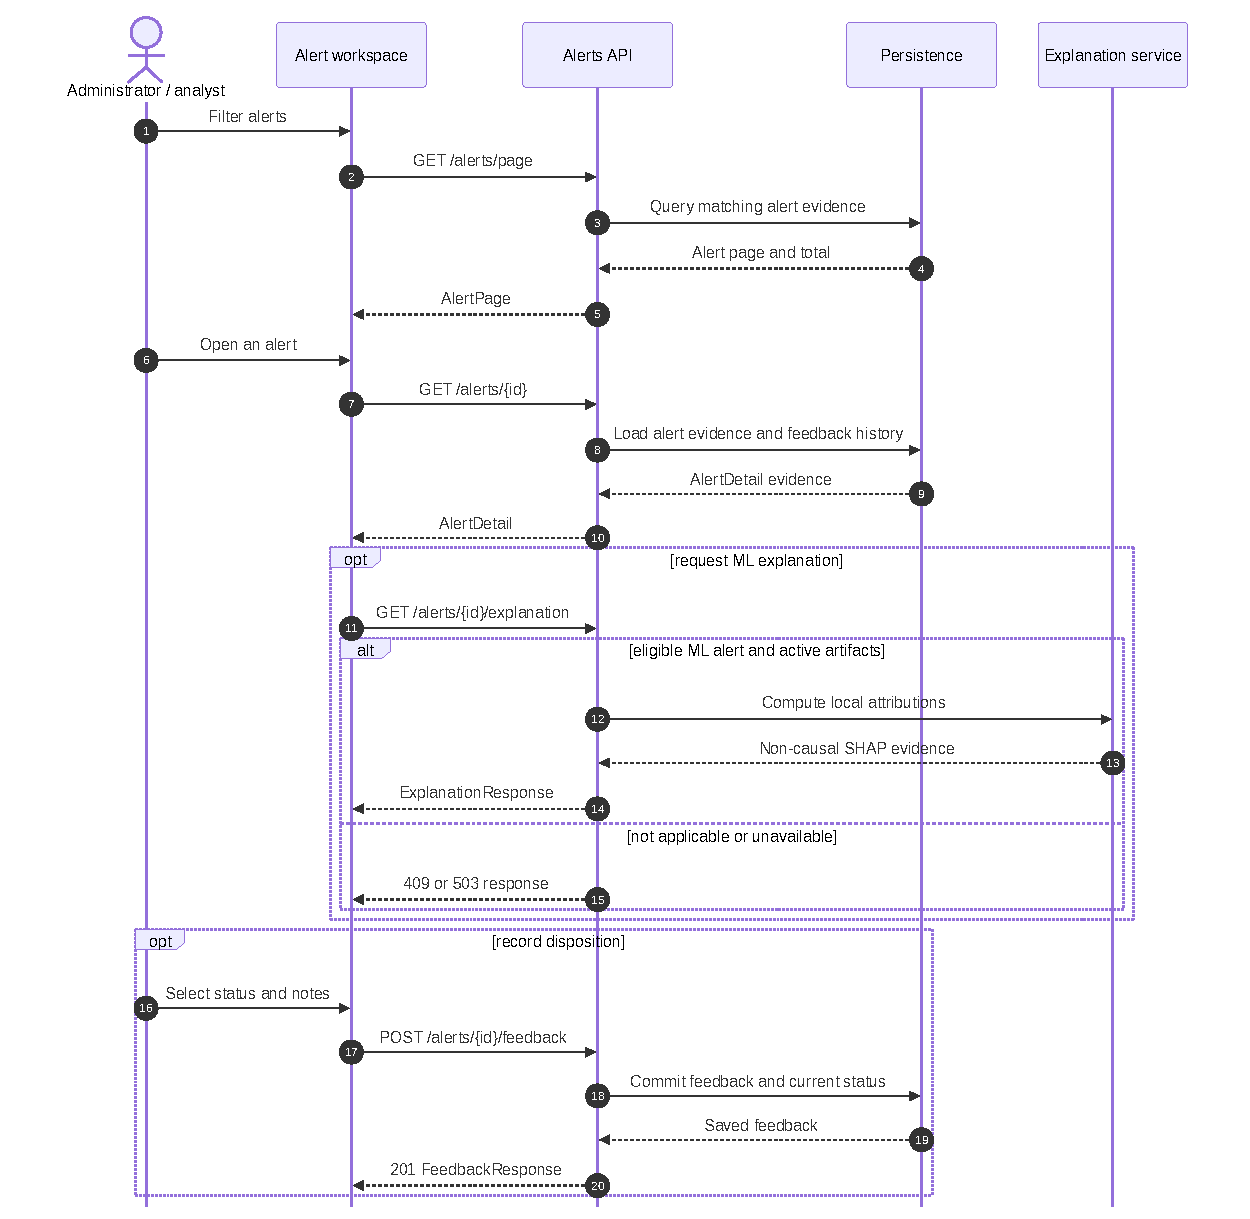
\includegraphics[width=\textwidth,height=0.68\textheight,keepaspectratio]{../diagrams/rendered/09-alert-investigation-sequence.pdf}
  \caption{S\'equence d'investigation et de qualification d'une alerte}
  \label{fig:alert-investigation}
\end{figure}

\clearpage
\subsection{Surveillance de la sant\'e des mod\`eles}

Le parcours de la figure~\ref{fig:model-health-sequence} rassemble les mesures
n\'ecessaires à l'examen d'un mod\`ele en service et à la restitution de son
\'etat dans l'interface d'administration.

\begin{figure}[htbp]
  \centering
  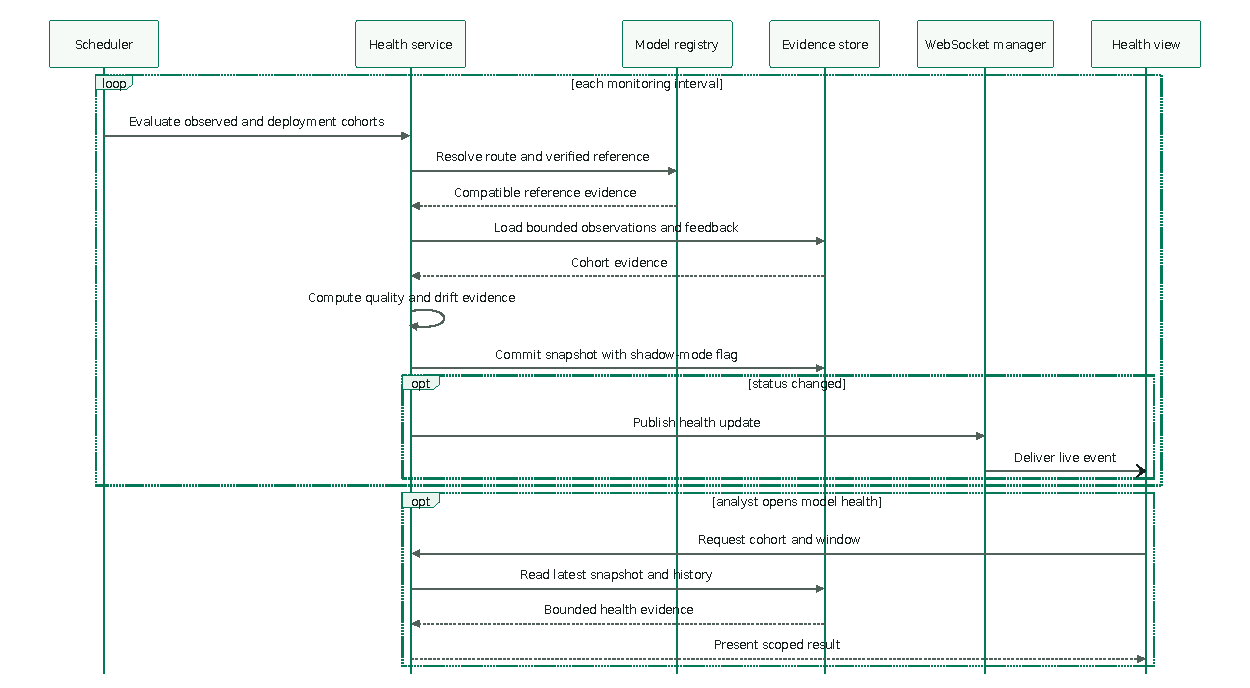
\includegraphics[width=\textwidth,height=0.68\textheight,keepaspectratio]{../diagrams/rendered/11-model-health-sequence.pdf}
  \caption{S\'equence de consultation de la sant\'e d'un mod\`ele}
  \label{fig:model-health-sequence}
\end{figure}

\subsection{Authentification, rejeu et capteur}

L'authentification précède l'accès aux fonctions protégées, comme l'exige
BF-01. Le rejeu applique le parcours de prédiction à une suite bornée de lignes
du jeu de données. L'agent Suricata dispose de sa propre route d'entrée : il
transmet des alertes de signature qui sont enregistrées puis publiées sans
appel aux modèles de classification.

\section{Conclusion}

La base relie les observations aux décisions et conserve les transitions des
travaux d'ingestion. Les services encadrent ces écritures par des transactions;
l'outbox reporte la publication après leur validation. Cette organisation
permet à l'interface de retrouver un résultat même si sa diffusion immédiate
a été interrompue.
